\section{Prospective relative-frequency prediction protocol}
\label{app:prediction}

\subsection{Observable, physical assumption, and fixed prediction}
\label{app:prediction_model}

This prospective design tests the apparent relative frequency of two Fe\,II
transitions, not a complete energy-level distribution.  The original
Riemann-motivated hypothesis concerns an additional uncertainty \emph{standard
deviation} proportional to $\ln^{-2}(t/t_*)$; it does not derive a mean line-centre
drift.  We explicitly add a universal deterministic mean response.  Testing
stochastic broadening instead would require independent atomic-response and
temporal/spatial-correlation models, and a separate protocol.  Failure of one
endpoint cannot be reinterpreted as success of the other.

The primary descriptor is fixed to
\begin{equation}
 D(z)=v_{2382}-v_{2374},\qquad Y_{\rm app}=-D/c.
 \label{app:descriptor}
\end{equation}
A common logarithmic-velocity zero point cancels, whereas differential
calibration, gas, isotope, and environmental effects remain.  A uniform
fractional rescaling of all transition frequencies can be absorbed into
redshift and is outside this test's sensitivity.

The age coordinate is a fixed flat matter--$\Lambda$ model with
$H_0=67.4\ {\rm km\,s^{-1}\,Mpc^{-1}}$, $\Omega_m=0.315$, and no radiation.
Set $t_0=t(0)$ and $t_*=5.391247\times10^{-44}\ {\rm s}$, using consistent time
units inside dimensionless logarithms.  Define
\begin{align}
 f_p(t)&=\left[\frac{\ln(t_0/t_*)}{\ln(t/t_*)}\right]^p-1,
 \label{app:time_function}\\
 H_p(z)&=\frac{f_p[t(z)]-f_p[t(1)]}{f_p[t(2)]-f_p[t(1)]},
 &D(z)&=b+B H_2(z).
 \label{app:endpoint_model}
\end{align}
Here $b=D(1)$ and $B=D(2)-D(1)$, in velocity units.  This normalization differs
from $D=b_{\rm old}+A G_2(z)$ with $G_p(z)=f_p[t(z)]/f_p[t(3)]$:
$B=0.312753948A$, with a corresponding intercept change.  Neither $B$ nor its
sign is currently predicted by the underlying hypothesis or measured by this
design calculation.  The cosmology, $t_*$, and primary exponent $p=2$ must not
be tuned using confirmation data.

At the illustrative design centres $z=(1,1.5,2)$, ages are
$(5.845622,4.264167,3.273357)$ Gyr and $H_2=(0,r,1)$, with
$r=0.542436444$.  Development estimates of the two endpoints therefore predict
a previously unexamined middle group:
\begin{equation}
 D(1.5)_{\rm pred}=0.457563556D(1)+0.542436444D(2).
 \label{app:midpoint_prediction}
\end{equation}
The hypothetical choice $B=100\ {\rm m\,s^{-1}}$ gives a middle-minus-low
contrast of $54.2436\ {\rm m\,s^{-1}}$; these are illustrative values, not
observations or theoretical amplitudes.  Actual predictions use each target's
redshift.  Group weights and averages of $H_2$ are frozen; applying $H_2$ to a
broad bin's mean redshift is not equivalent.

\subsection{Development, freezing, and independent confirmation}
\label{app:prediction_samples}

The existing seventeen ESPRESSO exposures and six archive candidates are
development material.  Future calibrated low- and high-redshift development
sightlines determine $b,B$, nuisance treatment, and predictive uncertainty.
An unconstrained or near-zero amplitude cannot yield a sharp nonzero
forecast.  Before accessing confirmation shifts, a public timestamped protocol
must fix target identities, selection and exclusion rules, code and data
versions, the fitted prediction and covariance, primary statistic and
threshold, bias budget, scientifically relevant $B_{\min}$, equivalence
tolerance, and stopping rules.  Current file hashes support reproducibility;
they do not constitute public preregistration.

Confirmation requires new independent sightlines in all three redshift
groups.  New endpoint targets replicate the nonzero contrast; a new midpoint
with old endpoints alone cannot do so.  Multiple absorbers on one sightline
share calibration uncertainty.  A provisional organization of four
development sightlines per endpoint and eight confirmation sightlines per
group totals 32, but establishes neither target availability nor adequate
power.  Final sample size follows blinded pilot precision and $B_{\min}$,
with at most one prespecified update using blinded quality/noise information,
never repeated additions until significance.

Zero- and nonzero-signal injections must cover gas architecture, response,
pixel covariance, optimization, and interval coverage.  Poor fit by a
constant-frequency model alone must not exclude a potentially shifted target;
failures follow frozen rules and remain reported.  Each redshift group needs
an independent-instrument subset, interleaved seasons/nights, and matched
absorption depth, width, saturation, and measurable environment.  Barycentric
velocity, trace, and valid overlapping-order controls test instrumental
stability.  Reobserving one absorber years later supplies no gigayear age
baseline; nearby-redshift independent sightlines instead constrain target
scatter.

\subsection{Prediction covariance and conventional-bias bounds}
\label{app:prediction_covariance}

For $\mathbf y=(D_L,D_M,D_H)^{\mathsf T}$, define
\begin{equation}
 C=\mathbf w^{\mathsf T}\mathbf y,
 \qquad\mathbf w=(-(1-r),1,-r)^{\mathsf T},
 \qquad\operatorname{Var}(C)=\mathbf w^{\mathsf T}\Sigma\mathbf w.
 \label{app:closure}
\end{equation}
For the frozen forecast, $L,H$ are development anchors and $M$ is new
confirmation data.  Closure among three new confirmation groups is an
additional shape diagnostic.  Crucially, $B=0$ also gives $C=0$: closure
cannot establish variation without independent nonzero endpoint replication.

The joint $\Sigma$ includes development uncertainty, validation errors, shared
laboratory references, calibration, sightlines, and trained models, including
cross-covariances.  Independent equal group errors $\sigma_g$ give
$\sigma_C=1.226214\sigma_g$ only as a special case.  A common laboratory
pair-zero covariance $\sigma_{\rm lab}^2\mathbf1\mathbf1^{\mathsf T}$ cancels
because $\mathbf w^{\mathsf T}\mathbf1=0$; wavelength distortions and
age-correlated environmental biases generally do not.

For arbitrary target redshifts, let $X=(1,H_2)$, with development and
validation subscripts $T,V$.  Fixed-covariance generalized least squares gives
\begin{align}
 M&=(X_T^{\mathsf T}\Sigma_{TT}^{-1}X_T)^{-1}
       X_T^{\mathsf T}\Sigma_{TT}^{-1},
 &\widehat{\boldsymbol\theta}&=M\mathbf y_T,
 \label{app:development_estimator}\\
 \mathbf e_V&=\mathbf y_V-X_VM\mathbf y_T.
 \label{app:validation_residual}
\end{align}
The predictive covariance is
\begin{equation}
 \begin{split}
 \Sigma_e={}&\Sigma_{VV}
 +X_VM\Sigma_{TT}M^{\mathsf T}X_V^{\mathsf T}\\
 &-\Sigma_{VT}M^{\mathsf T}X_V^{\mathsf T}
 -X_VM\Sigma_{TV}.
 \end{split}
 \label{app:full_prediction_covariance}
\end{equation}
Estimated covariance, model selection, or active bounds require full
injection-based coverage calibration, not an automatic exact $\chi^2$ claim.
Unknown bounded biases $|d_i|\leq\epsilon_i$ instead allow a closure bias up to
$\sum_i|w_i|\epsilon_i$, or $2\epsilon$ for equal bounds.  Structured biases
require maximization over their allowed set.  Such bounds must not be
silently converted into independent zero-mean Gaussian errors.

\subsection{Conditional power and instrument requirements}
\label{app:prediction_power}

Table~\ref{app:power_table} assumes eight confirmation targets per endpoint,
independent single-target random error $\sigma$, and known zero-mean Gaussian
group offsets of dispersion $\tau$, independent between groups.  Then
\begin{equation}
 \sigma_\Delta^2=2(\sigma^2/8+\tau^2).
 \label{app:power_variance}
\end{equation}
Correlated group offsets require the additional $-2\operatorname{Cov}$ term.
The two-sided $\alpha=0.01$ planning threshold neither calibrates unknown
systematics nor constitutes a discovery standard.

\begin{table}[tbp]
 \centering
 \caption{Hypothetical endpoint power for $|B|=100\ {\rm m\,s^{-1}}$ and
 eight targets per endpoint.  All velocity columns are in
 ${\rm m\,s^{-1}}$.  $|B|_{90\%}$ is the effect required for 90\% power under
 the stated known-Gaussian assumptions; no row represents measured performance.}
 \label{app:power_table}
 \begin{tabular}{rrrrr}
 \toprule
 $\sigma$ & $\tau$ & $\sigma_\Delta$ & Power & $|B|_{90\%}$\\
 \midrule
 50 & 10 & 28.72 & 81.7\% & 110.8\\
 100 & 20 & 57.45 & 20.2\% & 221.6\\
 200 & 30 & 108.63 & 4.9\% & 419.0\\
 \bottomrule
 \end{tabular}
\end{table}

The first scenario needs eleven targets per endpoint for 90\% power at
$|B|=100\ {\rm m\,s^{-1}}$, before development, midpoint, and replication
resources.  The other two cannot reach 90\% by increasing target numbers
alone because their group-error floors remain.

ESPRESSO covers 380--788 nm, with median HR resolving power approximately
140,000 \citep{ESOESPRESSO2026}.  The P117 manual places the current laser
frequency comb's blue end near 450 nm \citep{ESOESPRESSOManualP117}.
The proposed pair lies near 475/477, 594/596, and 712/715 nm; the high-redshift
windows require prior water-vapour screening.  The $z\simeq0.7$ pair is below
the current comb range and is excluded from this primary design.  HR plus
sky should be evaluated for faint quasars: the B fibre records sky or
Fabry--P\'erot, not both.  LFC/ThAr calibration is daytime operation, so
night-time comb exposures immediately bracketing science cannot be promised
\citep{ESOESPRESSOManualP117}.  Actual calibration chains and independent
drift/response constraints must be preserved; a science-fitted response is
not independent calibration.  Target-specific exposure-time calculations,
clean windows, and injection recovery precede any observing-hours claim.

\begin{figure}[tbp]
 \centering
 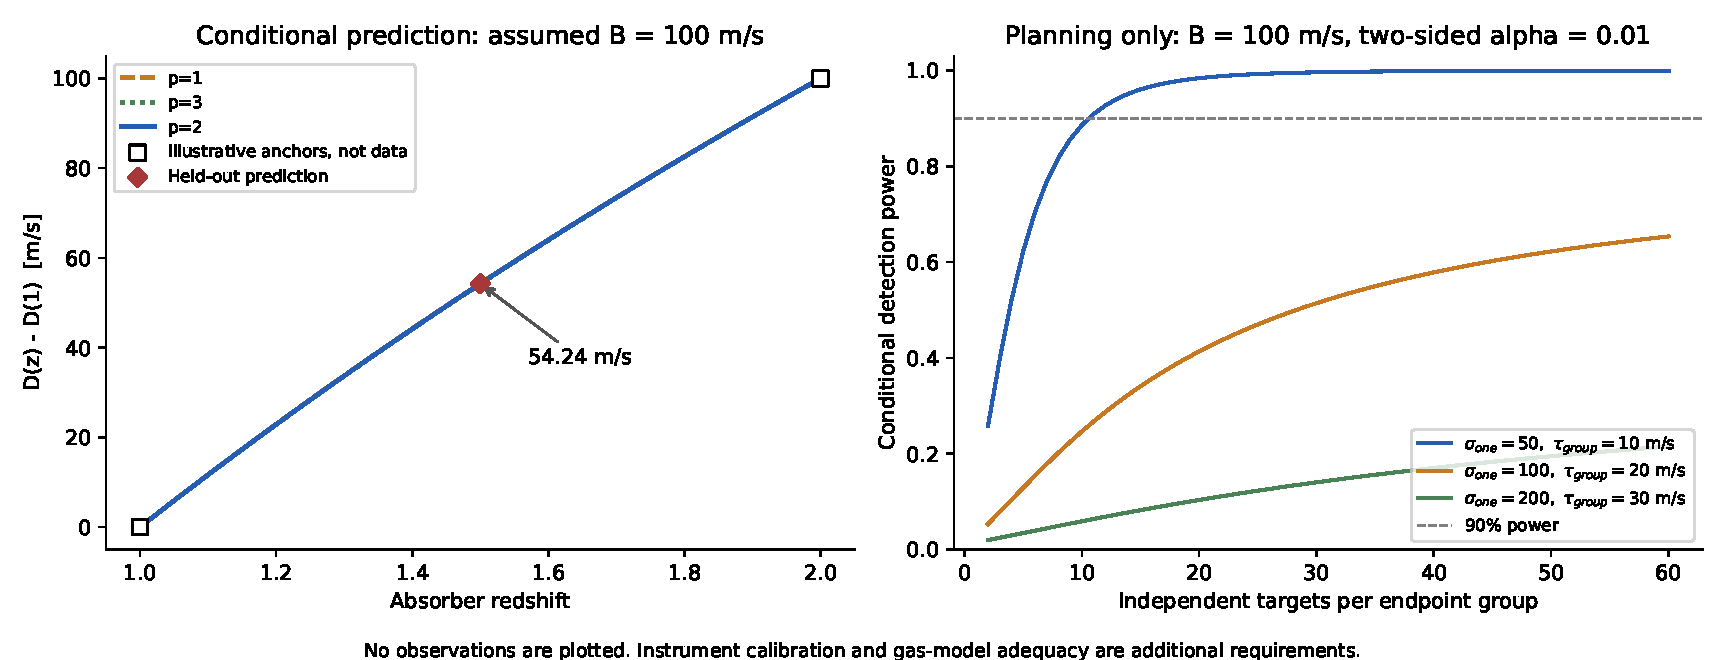
\includegraphics[width=0.98\textwidth,height=0.43\textheight,keepaspectratio]
 {../experiments/prediction_test_2026-09-21/figures/prediction_design.pdf}
 \caption{Conditional prediction geometry and hypothetical power calculations.
 There are no observed data points.  The displayed
 $B=100\ {\rm m\,s^{-1}}$ is illustrative; power assumes the stated Gaussian
 group-error floors and is not target-specific instrument performance.}
 \label{app:prediction_figure}
\end{figure}

\subsection{Failure criteria and scope of future conclusions}
\label{app:prediction_outcomes}

A replicated nonzero endpoint contrast, a sufficiently narrow interval
compatible with the frozen midpoint prediction, and successful conventional
controls would support the tested mean-response model over this sample range.
Adequate precision excluding its frozen direction or amplitude constitutes
failure of that prediction.  Midpoint disagreement implicates the shape,
universality, or measurement model; instrument-dependent shifts fail physical
attribution, and dominant same-age scatter requires environmental/gas checks.
Wide intervals covering both zero and the forecast are inconclusive.

Because $B=0$ remains allowed, a null result cannot exclude the whole
free-amplitude family.  A researcher-selected $B_{\min}$ is a relevance
threshold, not a theoretical lower bound.  Furthermore, after matching the
same endpoints at $B=100\ {\rm m\,s^{-1}}$, $p=1$ and $p=3$ alter the midpoint
by only approximately $+0.0517$ and $-0.0517\ {\rm m\,s^{-1}}$.  A detected
trend would therefore not identify $p=2$ or establish a Riemann origin.

As of 21 September 2026 this protocol is unregistered, with no frozen
amplitude, final qualified target list, allocated telescope time, or new
observations.  Existing instruments permit preparatory work; neither a
ten-year discovery nor an achievable precision is promised before target and
calibration qualification.
